\chapter[Avaliação de Capacidade]{Avaliação de Capacidade}
% ----------------------------------------------------------
Dadas as definições e formalizações propostas no anteriormente, faz-se necessária
a especificação de uma lógica de manipulação das entidades e operações descritas.

Passamos agora a descrever uma proposta de processo de avaliação de capacidade
que visa a buscar as Configurações de menor preço capazes de executar uma determinada 
Carga de Trabalho. Esse processo foi implementado como parte de um sistema 
computacional ao qual demos o nome de \emph{Cloud Capacitor} e que descreveremos 
no capítulo seguinte.  

\begin{figure}[htb]
  \caption{\label{fig_processo_alto_nivel}Visão geral do Processo de Avaliação de Capacidade}
  \begin{center}
    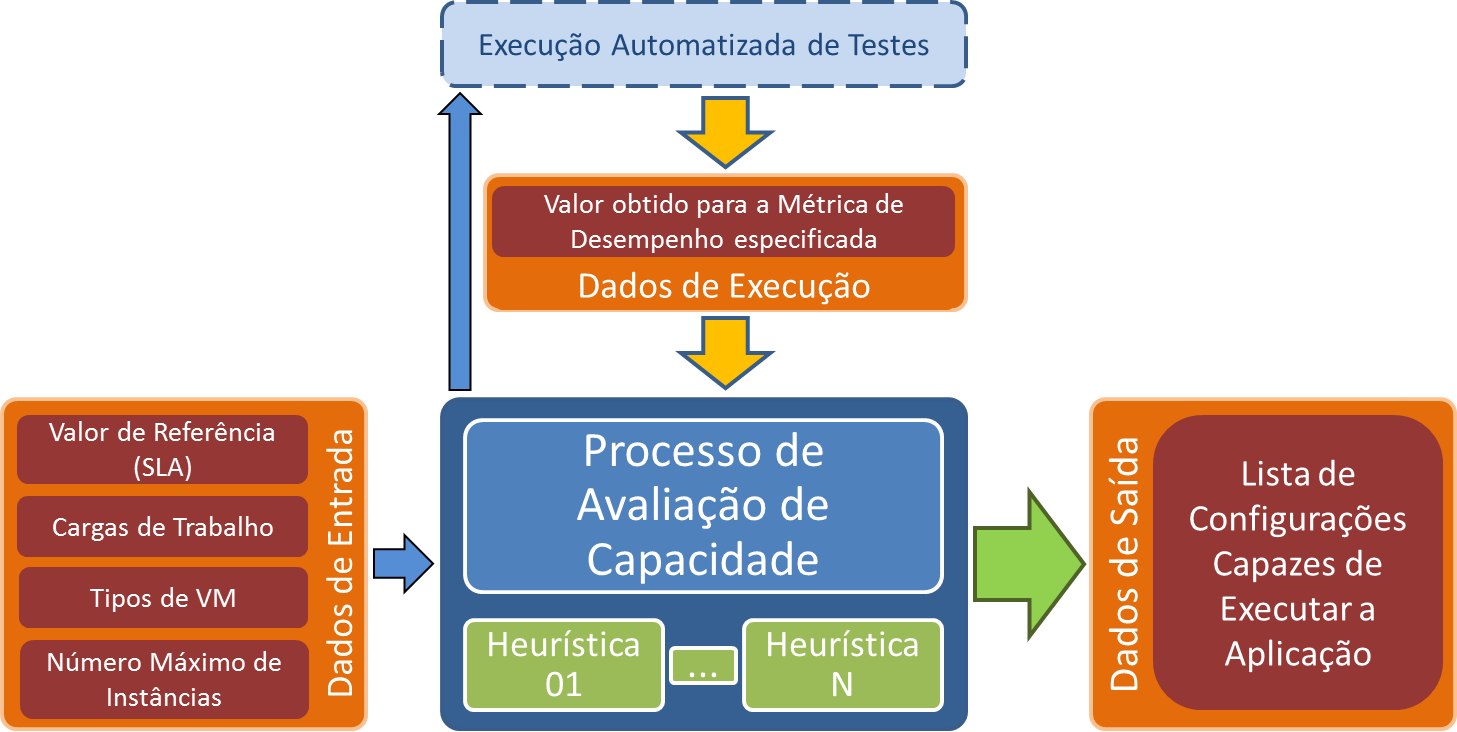
\includegraphics[scale=0.6]{img/processoAltoNivel}
  \end{center}
\end{figure}

O processo prevê um conjunto de dados de entrada, ao menos uma execução da 
Aplicação sob Teste no ambiente de nuvem de infraestrutura almejado para 
hospedá-la e a análise do desempenho obtido pela Aplicação a partir 
de suas execuções. Com base nos dados de desempenho, o processo passa por diversos
pontos de decisão que podem levar a novas execuções da Aplicação em diferentes 
cenários. Ao final do processo, é fornecida como saída uma lista de Configurações, 
ordenadas por preço, capazes de executar a Aplicação sob Cargas de Trabalho específicas.

Este capítulo estuda em detalhes todas as fases do processo 
proposto, explicando quais são os dados de entrada necessários, os componentes do 
processo e as operações pelas quais são responsáveis e quais as decisões pelas quais
o processo tem que passar até determinar quais são as Configurações de menor custo
capazes de executar a Aplicação.

\section{Dados de Entrada}

O principal parâmetro esperado pelo processo de avaliação de capacidade é o Valor
de Referência de Desempenho, ao qual também nos referimos como SLA 
(\emph{Service Level Agreement}). Esse valor será usadp para determinar 
se a Aplicação atingiu os requisitos mínimos de desempenho exigidos, conforme
veremos na descrição do funcionamento do processo, mais adiante.

Além do SLA, o processo precisa também conhecer quais são as Cargas de Trabalho
que deverão ser submetidas à Aplicação sob Teste durante seu funcionamento. Porém,
nem todas as Cargas de Trabalho serão submetidas de fato. Isso vai depender do 
conjunto de decisões tomadas pelo processo com base na comparação do desempenho 
da Aplicação com o SLA. Ainda assim, graças à sua característica de inferência de
desempenho, o processo mostra resultados para todas as Cargas de Trabalhado 
informadas como parâmetro de entrada.

Para que a Aplicação seja executada, é preciso que o processo conheça quais são
as Configurações disponibilizadas no Provedor de nuvem para esse fim. Para isso,
o processo deve ser alimentado com uma lista de Tipos de Máquinas Virtuais que
serão utilizadas na execução da Aplicação, bem como a quantidade máxima de 
instâncias usadas para compor cada Configuração. Através desses dados o processo
passa a conhecer então o Espaço de Implantação disponível para os testes de 
desempenho, composto por uma lista de Configurações geradas a partir da lista de
Tipos de Máquinas Virtuais disponíveis e do número máximo de instâncias.

\section{Funcionamento do Processo}

O processo de avaliação de capacidade proposto é um processo extensível, ao qual
devem ser ligados componentes para os quais são delegadas funções de cunho mais
específico, como a comunicação com o Provedor de nuvem e a Aplicação sob Teste
para fins de orquestração do teste de desempenho, e também funções para as quais
é desejado um certo grau de flexibilidade a fim de tornar o processo mais adaptável,
como a escolha das Cargas de Trabalho e Configurações que serão usadas na execução
da Aplicação.

Todas as atividades ligadas à rotina de execução da Aplicação, desde sua implantação,
passando pela criação e configuração das máquinas virtuais no ambiente do Provedor 
de nuvem, bem como pelo controle de inicialização e finalização dessas instâncias, 
serviços subjacentes como bancos de dados e filas, e a própria parametrização da 
execução e parada da Aplicação em si, não fazem parte do escopo do processo. Este,
por sua vez, presume que os dados de resultado para cada execução estarão disponíveis
quando necessários. A maneira como esses dados serão de fato obtidos é dependente
da implementação concreta do processo e é irrelevante do ponto de vista do seu 
funcionamento.  

Entretanto, o processo prevê a existência de um componente chamado Executor, que é 
o responsável pelas ações necessárias à execução da Aplicação sob Teste no ambiente
alvo. O Executor deve conhecer os detalhes inerentes à comunicação com o Provedor 
e com a Aplicação sob Teste e, assim, ser capaz de ordenar a sua execução e coletar
como resposta os dados de desempenho esperados pelo processo. O componente Executor
é um dos pontos de extensibilidade oferecidos pelo processo e sua implementação
concreta está fora do escopo deste trabalho, cujo foco não está na automação de
execução de testes de qualquer natureza.

\begin{figure}[hbt]
  \caption{\label{fig_processo_aval_capacidade}Diagrama de Funcionamento do Processo de Avaliação de Capacidade}
  \begin{center}
    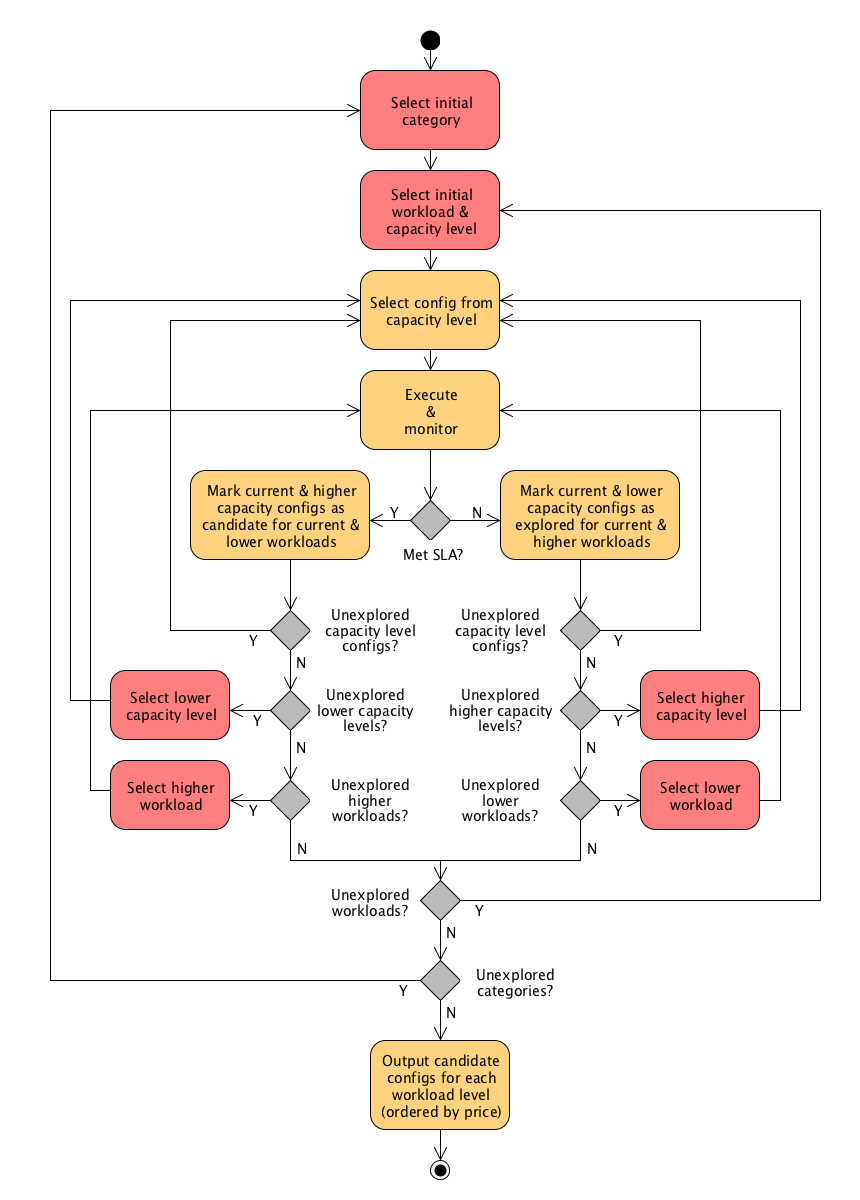
\includegraphics[scale=0.45]{img/diagrama-avaliacao-capacidade-v14}
  \end{center}
\end{figure}

Analogamente, as operações de seleção das Configuração sobre as quais a Aplicação
sob Teste será executada, bem como a seleção das Cargas de Trabalho a que ela 
será submetida durante sua execução, são delegadas a um componente que chamamos de
Estratégia de Avaliação ou, simplesmente, Estratégia. Seu objetivo é permitir a
aplicação de diferentes métodos para a escolha da melhor Configuração e/ou Carga 
de Trabalho mais adequada aos objetivos da avaliação de capacidade em curso e 
também ao perfil da Aplicação.

Dessa forma, o processo permite que a mesma Aplicação seja facilmente avaliada 
por meio de diferentes abordagens e sem modificação da lógica geral original de 
avaliação. Para exemplificar, uma Estratégia pode selecionar Configurações 
maiores ou menores priorizando a escalabilidade vertical em detrimento da mudança
do número de instâncias que compõem a Configuração anterior. Outra Estratégia 
poderia agir priorizando a escolha de máquinas mais robustas ou cargas de trabalho
maiores quando o SLA informado fosse mais folgado.

De modo contrário em relação ao Executor, a definição de Estratégias de Avaliação
está intrinsecamente ligada aos objetivos deste trabalho de estudar os efeitos da
inferência de desempenho na eficiência do processo de avaliação de capacidade para
aplicações em ambientes de nuvem de infraestrutura. A inteligência das Estratégias
propostas, ou seja, sua capacidade de escolher corretamente as Configurações e 
Cargas de Trabalho, é determinante para o sucesso do processo e da técnica de 
inferência. 

Para efeito de entendimento do funcionamento geral do processo de avaliação de 
capacidade ora proposto, podemos abstrair temporariamente o comportamento da 
Estratégia de Avaliação, o qual voltaremos a analisar um pouco mais adiante. 
Esta é, aliás, outra vantagem da abordagem adotada de delegação de funções 
específicas a componentes: além da flexibilidade e adaptabilidade, a abstração 
dessas operações torna mais fáceis o entendimento, a descrição e a implementação 
concreta do processo.   

Na Figura~\ref{fig_processo_aval_capacidade}, os blocos em vermelho representam
as operações que o processo espera que sejam executadas por uma Estratégia de 
Avaliação. Os outros blocos referem-se a ações comuns do próprio processo, 
executadas de maneira idêntica independentemente de qual seja a Aplicação sob Teste
ou de qual seja a Estratégia de Avaliação usada. A delegação de funções para o 
componente Executor não está destacada no diagrama e se dá no passo 
``\emph{Execute \& Monitor}'', situado aproximadamente no centro da figura.

\subsection{Operações iniciais}
Uma vez tendo recebido os dados de entrada, o processo tem seu início com as 
primeiras invocações da Estratégia utilizada na avaliação. É o momento de escolher
por onde começar a execução dos testes.

A primeira atividade delegada pelo processo à Estratégia é a escolha da Categoria 
inicial. Conforme as definições apresentadas no Capítulo 3, os Tipos de Máquinas
Virtuais oferecidos pelo Provedor são normalmente agrupadas por Categorias, que
reunem máquinas de propósito e atributos semelhantes. Assim, o Espaço de Implantação
sobre o qual a avaliação de capacidade se dará está dividido em Categorias. O número 
de Categorias envolvidas na avaliação depende do conjunto de máquinas virtuais
selecionados pelo usuário e passados como parte dos dados de entrada do processo.

Assim, como primeiro passo no processo de avaliação, e Estratégia seleciona, 
segundo sua própria lógica, dependente de implementação, qual a primeira
Categoria de máquinas a ser explorada.

Depois de escolhida a Categoria inicial, a Estratégia é solicitada a escolher 
qual a primeira Carga de Trabalho a ser imposta sobre a Aplicação sob Teste. Essa 
escolha também é feita conforme a lógica própria da Estratégia e deve selecionar
o volume de trabalho inicial a partir da lista de Cargas fornecida nos dados de 
entrada.

\subsubsection{Níveis de Capacidade}
Dando continuidade à sequência de operações iniciais dentro do Processo de Avaliação 
de Capacidade, a Estratégia deve selecionar um Nível de Capacidade inicial. 

Níveis de Capacidade são um conceito criado para ajudar a estabelecer uma hierarquia 
sobre as relações de capacidade de processamento entre as diversas Configurações. 
Essa hierarquia de capacidade é válida apenas entre Configurações de uma mesma 
Categoria de Máquinas Virtuais. 

\begin{figure}[hbt]
  \caption{\label{fig_niveis_capacidade}Agrupamento de Configurações por Níveis de Capacidade}
  \begin{center}
    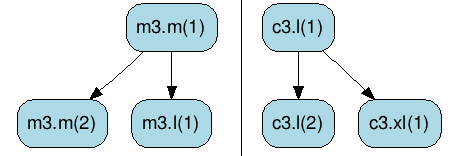
\includegraphics{img/exemplo-niveis-capacidade}
  \end{center}
\end{figure}

Para cada Categoria, o Nível "um" de Capacidade é composto apenas pela Configuração 
de menor preço dentro da Categoria. Um novo nível é criado com todas as Configurações 
para as quais é verdadeira a relação "maior que", conforme a definição descrita 
no Seção 3.2.5. Esse então passa a ser o Nível "dois" e a lógica se repete daí em diante, 
tomando-se, para cada Configuração desse nível, as imediatamente maiores, 
formando um novo Nível. O procedimento continua até que todas as Configurações 
estejam devidamente classificadas em Níveis de Capacidade.

A Figura~\ref{fig_niveis_capacidade} mostra um pequeno exemplo, onde 6 Configurações
pertencentes a duas Categorias distintas foram classificadas em dois Níveis de 
Capacidade dentro de cada Categoria. Os retângulos representam as Configurações, 
com o nome do Tipo de Máquina Virtual utilizado e o número entre parênteses 
representa a quantidade de instâncias que compõem a Configuração. As setas que 
ligam as Configurações indicam a relação de capacidade entre elas apontando da 
menor para a maior. A ausência de seta entre duas Configurações implica a 
impossibilidade de se afirmar uma relação de capacidade entre elas. 

Assim, observando o Espaço de Implantação organizado por Categorias e classificado
hierarquicamente, a Estratégia deve selecionar, com base em sua própria lógica, um
Nível de Capacidade inicial. As Configurações que fazem parte do Nível inicial 
escolhido são disponibilizadas para que a Avaliação proceda com a execução dos 
testes da Aplicação.

\subsubsection{Ciclo de Execução de Testes}
Após a escolha da Carga de Trabalho inicial e do primeiro Níveç de Capacidade a
ser avaliado, o processo entra em um laço. 

De maneira geral, toma-se uma Configuração a partir do Nível de Capacidade atual, 
executa-se a Aplicação sob Teste impondo-se a ela a Carga de Trabalho selecionada 
e analisa-se o resultado dessa execução. O processo então se bifurca no primeiro
ponto de decisão, comparando o valor obtido pela Aplicação para a Métrica de 
Desempenho com o SLA definido nos dados de entrada.

Se o desempenho da Aplicação satisfaz o SLA proposto, o Processo considera que a
Configuração é capaz de executar sob a Carga de Trabalho imposta e sob todas as
Cargas de Trabalho menores. Além disso, o Processo infere que todas as 
Configurações maiores que a atual, da mesma maneira, podem executar
a Aplicação sob a Carga de Trabalho atual e também sob as Cargas menores. 

Caso o desempenho da Aplicação não satisfaça o SLA, o Processo considera que a 
Configuração não é capaz de executar sob a Carga de Trabalho atual e nem sob as
Cargas maiores. O Processo infere então que as Configurações menores igualmente
não serão capazes de executar sob a Carga atual e tampouco sob as de maior volume.

O Processo atinge então mais um ponto de decisão. Se existirem Configurações
pertencentes ao atual Nível de Capacidade cujas execuções ainda não tenham sido 
avaliadas para a Carga de Trabalho selecionada, o Processo volta ao passo de 
seleção de uma Configuração a partir do Nível de Capacidade e uma nova execução
é solicitada ao componente Executor.

Se não existirem Configurações inexploradas para a Carga de Trabalho atual no
Nível de Capacidade corrente, o Processo buscará por um Nível de Capacidade que 
ainda não tenha sido completamente explorado. Se a Aplicação satisfez o SLA na 
execução anterior, a Estratégia deverá selecionar um Nível de Capacidade menor. 
Se o SLA não tiver sido atingido, a Estratégia tentará selecionar um  Níveç de 
Capacidade maior. Depois de selecionado o próximo Nível de Capacidade, o laço do
Processo retorna ao ponto de seleção da próxima Configuração e outra execução 
acontece.
   
Novo ponto de decisão surge quando a Estratégia não encontra um Nível de 
Capacidade a ser explorado. Nessa situação, a Estratégia deve buscar uma Carga 
de Trabalho que não tenha sido avaliada. Se a execução anterior atingiu o SLA,
uma Carga de Trabalho maior será buscada. Caso contrário, a Estratégia tentará
uma Carga menor que a atualmente selecionada. Porém, se a Estratégia não conseguir 
fornecer uma Carga de Trabalho segundo essas restrições, o processo tentará a 
escolha de uma Carga inexplorada qualquer, bem como um Nível de Capacidade que 
disponha de pelo menos uma Configuração inexplorada, mesmo que de outra Categoria.    

Caso não seja encontrada uma Carga e nem um Nível de Capacidade, o Processo de 
Avaliação está terminado e é fornecida, para cada Carga de Trabalho, uma lista 
de Configurações, em ordem crescente de preço, capazes de executar a Aplicação 
sob Teste.  

\section{Resumo}
Apresentamos neste capítulo uma proposta de processo de avaliação de capacidade
cuja ideia chave é a inferência de capacidade de um recurso a partir dos dados 
reais de desempenho obtidos por um outro recurso semelhante, mas de capacidade
presumidamente menor ou maior.

Essa proposta de processo se apoia na hipótese de que é possível estabelecer uma
relação de capacidade entre os recursos disponibilizados por um provedor de nuvem
de infraestrutura. Com base nessa hipótese, criamos uma sequência de passos que
visam a identificar quais recursos são capazes de executar uma determinada 
aplicação sob determinados volumes de carga de trabalho com o menor número
possível de execuções reais da aplicação. Como resultado, o processo busca
a redução de custo e tempo normalmente envolvidos na atividade de avaliação de
capacidade dos recursos disponíveis na nuvem.

No Capítulo 5 a seguir apresentaremos uma visão mais concreta, com a descrição do 
arcabouço de software desenvolvido neste trabalho como implementação de referência
para o processo proposto. Apresentaremos também uma aplicação
web desenvolvida utilizando o arcabouço com o intuito de atestar a efetividade do processo de avaliação 
de capacidade baseado em inferência de desempenho. Essa aplicação foi usada para
demonstração da criação de algumas Estratégias criadas e para a execução dos 
testes de eficácia e efetividade das técnicas propostas, bem como das próprias
Estratégias, e cujos resultados apresentaremos no Capítulo 6 mais adiante.
   
% ----------------------------------------------------------
